\section{子问题的求解}
\label{sec:tr-subproblem}

第~\ref{sec:tr-model}节的刻画需要分解$\bm{B}+\lambda\bm{I}$好几次，每一轮外层迭代都这样做，代价可能比外层本身还高。接下来要弄清：能否用便宜得多的办法得到一个“够用”的步？

下面对同一个模型和同一个半径比较三种计算。它们是：只沿负梯度取步、把负梯度步与Newton步连起来、用共轭梯度迭代逐步逼近。主例取点$\bm{a}$的数据~\eqref{eq:tr-data-a}，半径$\Delta=2$；Hessian不定的情形用原点的数据~\eqref{eq:tr-data-o}。外层迭代真正需要的，不是子问题的精确解，而是模型下降达到一个规定的比例。这个比例由最简单的那种步来给出。

本节所有量都在同一轮外层迭代内，省略上标$(t)$，写$m,\bm{g},\bm{B},\Delta$。

\subsection{Cauchy步}
\label{sec:tr-cauchy}

\paragraph{沿负梯度最小化模型}
最便宜的做法是只在负梯度这条射线上找模型的最小点。设$\bm{g}\neq\bm{0}$，把点写成$\bm{p}=-a\,\bm{g}/\lVert\bm{g}\rVert_2$，其中$a\in[0,\Delta]$是走过的长度。令
\[
 \kappa=\frac{\bm{g}^\top\bm{B}\bm{g}}{\lVert\bm{g}\rVert_2^2},
\]
它是模型沿负梯度方向的曲率。代入式~\eqref{eq:tr-model}，模型的变化量是一元二次函数
\begin{equation}
 \psi(a)=m\Bigl(-a\frac{\bm{g}}{\lVert\bm{g}\rVert_2}\Bigr)-m(\bm{0})=-a\lVert\bm{g}\rVert_2+\frac{\kappa}{2}a^2.
 \label{eq:tr-cauchy-psi}
\end{equation}

在$[0,\Delta]$上最小化$\psi$，分两种情形。若$\kappa\leq0$，$\psi$严格递减，应当走到边界$a=\Delta$。若$\kappa>0$，$\psi$的顶点在$a=\lVert\bm{g}\rVert_2/\kappa$，它在区间内就取顶点，否则截断在边界。合起来就得到\term{Cauchy步}（Cauchy step）的长度，步本身记为$\bm{p}^{\mathrm{C}}$：
\begin{equation}
 \bm{p}^{\mathrm{C}}=-a^{\mathrm{C}}\frac{\bm{g}}{\lVert\bm{g}\rVert_2},\qquad
 a^{\mathrm{C}}=
 \begin{cases}
  \Delta,&\kappa\leq0,\\
  \min\{\Delta,\ \lVert\bm{g}\rVert_2/\kappa\},&\kappa>0.
 \end{cases}
 \label{eq:tr-cauchy-step}
\end{equation}
图~\ref{fig:tr-cauchy-cases}画出三种情形。计算时只需要一次矩阵向量乘积$\bm{B}\bm{g}$。

\begin{BookInlineFigure}
 \centering
 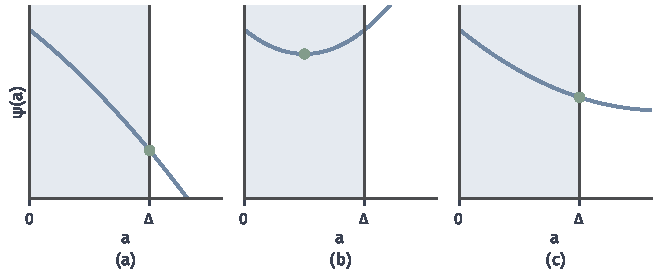
\includegraphics[width=112mm]{figures/05-optimization/02-smooth-optimization/matplotlib/tr-cauchy-cases/figure.pdf}
 \caption{函数$\psi(a)$（蓝）的三种情形，浅蓝带是可取的范围，深灰线是边界，绿点是Cauchy步的长度。(a)~$\kappa\leq0$，走到边界。(b)~$\kappa>0$且顶点在区间内，取顶点。(c)~$\kappa>0$但顶点在区间外，截断在边界。}
 \label{fig:tr-cauchy-cases}
\end{BookInlineFigure}

点$\bm{a}$的数据上，$\bm{g}^\top\bm{B}\bm{g}=49\times14=686$，$\lVert\bm{g}\rVert_2^2=98$，所以
\[
 \kappa=7,\qquad\lVert\bm{g}\rVert_2=7\sqrt2,\qquad\frac{\lVert\bm{g}\rVert_2}{\kappa}=\sqrt2.
\]

半径$\Delta=2$大于$\sqrt2$，Cauchy步取顶点：
\[
 \bm{p}^{\mathrm{C}}=-\sqrt2\cdot\frac{(7,7)^\top}{7\sqrt2}=\begin{bmatrix}-1\\-1\end{bmatrix},\qquad
 \operatorname{pred}(\bm{p}^{\mathrm{C}})=7\sqrt2\cdot\sqrt2-\frac72\cdot2=7.
\]
半径若取$\Delta=1$，则截断在边界，$a^{\mathrm{C}}=1$，预测下降为$7\sqrt2-3.5\approx6.40$。

\paragraph{Cauchy步提供的模型下降}
Cauchy步便宜，它的价值却在于给出了一条有保证的下限。下面的引理说明，它的预测下降由梯度大小、半径和曲率上界控制。

\begin{lemma}[Cauchy步的下降量]
 \label{lem:tr-cauchy-decrease}
 设$\bm{g}\neq\bm{0}$，$\bm{B}$对称。Cauchy步满足
 \begin{equation}
  \operatorname{pred}(\bm{p}^{\mathrm{C}})\geq\frac12\lVert\bm{g}\rVert_2\min\Bigl\{\Delta,\ \frac{\lVert\bm{g}\rVert_2}{\lVert\bm{B}\rVert_2}\Bigr\},
  \label{eq:tr-cauchy-decrease}
 \end{equation}
 其中$\bm{B}=\bm{0}$时第二项理解为$+\infty$。
\end{lemma}

\begin{proof}
 由式~\eqref{eq:tr-cauchy-psi}，预测下降是
 \[
  \operatorname{pred}(\bm{p}^{\mathrm{C}})=a^{\mathrm{C}}\lVert\bm{g}\rVert_2-\frac{\kappa}{2}(a^{\mathrm{C}})^2,
 \]
 并且$\kappa\leq\lVert\bm{B}\rVert_2$。按三种情形估计。

 若$\kappa\leq0$，则$a^{\mathrm{C}}=\Delta$，第二项非负，所以
 \[
  \operatorname{pred}(\bm{p}^{\mathrm{C}})\geq\Delta\lVert\bm{g}\rVert_2.
 \]

 若$\kappa>0$且$\lVert\bm{g}\rVert_2/\kappa\leq\Delta$，则取顶点，所以
 \[
  \operatorname{pred}(\bm{p}^{\mathrm{C}})=\frac{\lVert\bm{g}\rVert_2^2}{2\kappa}\geq\frac{\lVert\bm{g}\rVert_2^2}{2\lVert\bm{B}\rVert_2}.
 \]

 若$\kappa>0$且$\lVert\bm{g}\rVert_2/\kappa>\Delta$，则$a^{\mathrm{C}}=\Delta$，并且$\kappa\Delta<\lVert\bm{g}\rVert_2$，所以
 \[
  \operatorname{pred}(\bm{p}^{\mathrm{C}})=\Delta\lVert\bm{g}\rVert_2-\frac{\kappa\Delta}{2}\Delta\geq\frac12\Delta\lVert\bm{g}\rVert_2.
 \]
 三种情形都不小于式~\eqref{eq:tr-cauchy-decrease}的右端。
\end{proof}

点$\bm{a}$的数据上$\lVert\bm{B}\rVert_2=11$，取$\Delta=2$，式~\eqref{eq:tr-cauchy-decrease}的右端是
\[
 \frac12\cdot7\sqrt2\cdot\min\Bigl\{2,\ \frac{7\sqrt2}{11}\Bigr\}=\frac{49}{11}\approx4.45,
\]
确实不超过实际的预测下降$7$。这个下限比实际值松，它的用处在于对所有模型一致成立。

这条下限只用到一阶信息和曲率的上界，$\bm{B}$可以不定。我们把它提升为对任意候选步的要求：若存在常数$c_1\in(0,1]$，使得
\begin{equation}
 \operatorname{pred}(\bm{p})\geq c_1\lVert\bm{g}\rVert_2\min\Bigl\{\Delta,\ \frac{\lVert\bm{g}\rVert_2}{\lVert\bm{B}\rVert_2}\Bigr\},
 \label{eq:tr-sufficient-decrease}
\end{equation}
就说$\bm{p}$达到\term{充分模型下降}（sufficient model decrease）。第~\ref{sec:tr-convergence}节会看到，一阶收敛只需要这一条；任何预测下降不低于Cauchy步的求解器，都自动满足它，$c_1=1/2$。

要分清这条保障和精确求解的差别。式~\eqref{eq:tr-sufficient-decrease}只是一条下限，并不表示接近子问题的最优值。点$\bm{a}$上Cauchy步的预测下降是$7$，全局解是$10.115$；原点上$\Delta=2$时，Cauchy步是$1$，全局解是$4.111$。只用Cauchy步的方法本质上是最速下降，保留了收敛性，也保留了最速下降的慢。下面两种办法都从它出发，再往前走。

\subsection{狗腿法}
\label{sec:tr-dogleg}

\paragraph{主要思想}
设$\bm{B}\succ\bm{0}$。半径很小时，子问题的解贴近负梯度方向；半径足够大时，解就是Newton点。图~\ref{fig:tr-line-vs-region}中的绿线连接着这两端。求这条曲线要解久期方程，代价较高，\term{狗腿法}（dogleg method）用两段折线代替它。

折线的三个端点是原点、模型沿负梯度的最小点，以及Newton点：
\begin{equation}
 \bm{p}^{\mathrm{U}}=-\frac{\bm{g}^\top\bm{g}}{\bm{g}^\top\bm{B}\bm{g}}\bm{g},\qquad
 \bm{p}^{\mathrm{N}}=-\bm{B}^{-1}\bm{g}.
 \label{eq:tr-dogleg-points}
\end{equation}
上标U表示无约束（unconstrained）。用$\tau\in[0,2]$作路径的参数：
\begin{equation}
 \bm{p}(\tau)=
 \begin{cases}
  \tau\,\bm{p}^{\mathrm{U}},&0\leq\tau\leq1,\\
  \bm{p}^{\mathrm{U}}+(\tau-1)(\bm{p}^{\mathrm{N}}-\bm{p}^{\mathrm{U}}),&1\leq\tau\leq2.
 \end{cases}
 \label{eq:tr-dogleg-path}
\end{equation}

狗腿法在这条路径上走，走到半径为止。这样做合理，要靠路径的两个性质：沿路径越走越远，模型值也越走越低。前者保证路径与球面至多相交一次，后者保证交点是路径上模型最低的可行点。图~\ref{fig:tr-dogleg-monotone}是点$\bm{a}$上的这两条曲线，下面的引理给出证明。

\begin{BookInlineFigure}
 \centering
 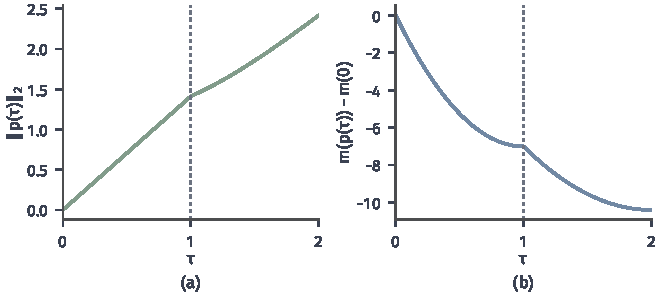
\includegraphics[width=112mm]{figures/05-optimization/02-smooth-optimization/matplotlib/tr-dogleg-monotone/figure.pdf}
 \caption{点$\bm{a}$的数据上沿狗腿路径的两个量，虚线$\tau=1$是折点$\bm{p}^{\mathrm{U}}$。(a)~长度严格增加。(b)~模型值严格减小。}
 \label{fig:tr-dogleg-monotone}
\end{BookInlineFigure}

\begin{lemma}[狗腿路径的单调性]
 \label{lem:tr-dogleg-monotone}
 设$\bm{B}\succ\bm{0}$，$\bm{g}\neq\bm{0}$。沿路径~\eqref{eq:tr-dogleg-path}，$\lVert\bm{p}(\tau)\rVert_2$单调不减，$m(\bm{p}(\tau))$单调不增。
\end{lemma}

\begin{proof}
 第一段上$\bm{p}$是从原点出发的线段，长度递增；$\bm{p}^{\mathrm{U}}$是模型沿这条射线的最小点，模型值递减。

 第二段记$\bm{w}=\bm{p}^{\mathrm{N}}-\bm{p}^{\mathrm{U}}$，$s=\tau-1\in[0,1]$。先看模型值。$h(s)=m(\bm{p}^{\mathrm{U}}+s\bm{w})$是凸二次函数，它在$s=1$处的导数是
 \[
  h'(1)=\langle\bm{B}\bm{p}^{\mathrm{N}}+\bm{g},\bm{w}\rangle=0,
 \]
 因为$\bm{B}\bm{p}^{\mathrm{N}}=-\bm{g}$。凸函数的导数单调不减，所以在$[0,1]$上$h'\leq0$。

 再看长度。$\tfrac12\lVert\bm{p}^{\mathrm{U}}+s\bm{w}\rVert_2^2$对$s$的导数是$\langle\bm{p}^{\mathrm{U}},\bm{w}\rangle+s\lVert\bm{w}\rVert_2^2$，只需证$\langle\bm{p}^{\mathrm{U}},\bm{w}\rangle\geq0$。记$\tau_{\mathrm{U}}>0$为式~\eqref{eq:tr-dogleg-points}中$\bm{g}$前的系数，代入该式，得到
 \[
  \langle\bm{p}^{\mathrm{U}},\bm{w}\rangle=\tau_{\mathrm{U}}\,\bm{g}^\top\bm{B}^{-1}\bm{g}-\tau_{\mathrm{U}}^2\,\bm{g}^\top\bm{g}
  =\frac{\tau_{\mathrm{U}}\bigl[(\bm{g}^\top\bm{B}^{-1}\bm{g})(\bm{g}^\top\bm{B}\bm{g})-(\bm{g}^\top\bm{g})^2\bigr]}{\bm{g}^\top\bm{B}\bm{g}}.
 \]
 取$\bm{u}=\bm{B}^{1/2}\bm{g}$，$\bm{v}=\bm{B}^{-1/2}\bm{g}$，方括号就是$\lVert\bm{u}\rVert_2^2\lVert\bm{v}\rVert_2^2-\langle\bm{u},\bm{v}\rangle^2$，由Cauchy--Schwarz不等式非负。
\end{proof}

\paragraph{计算过程}
下面用点$\bm{a}$的数据~\eqref{eq:tr-data-a}、半径$\Delta=2$走一遍。

需要的量是梯度$\bm{g}\in\mathbb{R}^n$、对称正定矩阵$\bm{B}\in\mathbb{R}^{n\times n}$、半径$\Delta$，输出位移$\bm{p}$。例中已知$\bm{g}=(7,7)^\top$，$\bm{B}=\operatorname{diag}(11,3)$。步骤如下。

\begin{enumerate}
 \item 由式~\eqref{eq:tr-dogleg-points}计算Newton点，若$\lVert\bm{p}^{\mathrm{N}}\rVert_2\leq\Delta$，返回$\bm{p}=\bm{p}^{\mathrm{N}}$。例中
 \[
  \bm{p}^{\mathrm{N}}=\begin{bmatrix}-7/11\\-7/3\end{bmatrix},\qquad\lVert\bm{p}^{\mathrm{N}}\rVert_2\approx2.419>2,
 \]
 所以继续。
 \item 由式~\eqref{eq:tr-dogleg-points}计算$\bm{p}^{\mathrm{U}}$，若$\lVert\bm{p}^{\mathrm{U}}\rVert_2\geq\Delta$，返回边界上的负梯度步$\bm{p}=-\Delta\bm{g}/\lVert\bm{g}\rVert_2$，这就是Cauchy步。例中
 \[
  \bm{p}^{\mathrm{U}}=-\frac{98}{686}\begin{bmatrix}7\\7\end{bmatrix}=\begin{bmatrix}-1\\-1\end{bmatrix},\qquad\lVert\bm{p}^{\mathrm{U}}\rVert_2=\sqrt2<2,
 \]
 所以继续。
 \item 否则交点在第二段上。记$\bm{w}=\bm{p}^{\mathrm{N}}-\bm{p}^{\mathrm{U}}$，解$\lVert\bm{p}^{\mathrm{U}}+s\bm{w}\rVert_2=\Delta$的正根：
 \begin{equation}
  s=\frac{-\langle\bm{p}^{\mathrm{U}},\bm{w}\rangle+\sqrt{\langle\bm{p}^{\mathrm{U}},\bm{w}\rangle^2+\lVert\bm{w}\rVert_2^2\bigl(\Delta^2-\lVert\bm{p}^{\mathrm{U}}\rVert_2^2\bigr)}}{\lVert\bm{w}\rVert_2^2}.
  \label{eq:tr-boundary-root}
 \end{equation}
 例中$\bm{w}=(4/11,\,-4/3)^\top$，三个系数是
 \[
  \lVert\bm{w}\rVert_2^2=\frac{2080}{1089},\qquad\langle\bm{p}^{\mathrm{U}},\bm{w}\rangle=\frac{1056}{1089},\qquad\Delta^2-\lVert\bm{p}^{\mathrm{U}}\rVert_2^2=2.
 \]
 根号内的量是$(2376/1089)^2$，因此
 \[
  s=\frac{-1056+2376}{2080}=\frac{33}{52}.
 \]
 \item 返回$\bm{p}=\bm{p}^{\mathrm{U}}+s\bm{w}$。例中
 \[
  \bm{p}=\begin{bmatrix}-1+3/13\\-1-11/13\end{bmatrix}=\begin{bmatrix}-10/13\\-24/13\end{bmatrix},
 \]
 长度恰为$\sqrt{100+576}/13=2$。
\end{enumerate}

最终得到的预测下降是
\[
 \operatorname{pred}(\bm{p})=\frac{238}{13}-\frac{1414}{169}=\frac{1680}{169}\approx9.941.
\]
这已经是全局解$10.115$的$98\%$，而全局解要解一元非线性方程。图~\ref{fig:tr-dogleg-path}给出三种半径下的结果：$\Delta=1$时只用到第一段，$\Delta=2$时落在第二段，$\Delta=3$时完整的Newton步被采用。

\begin{BookInlineFigure}
 \centering
 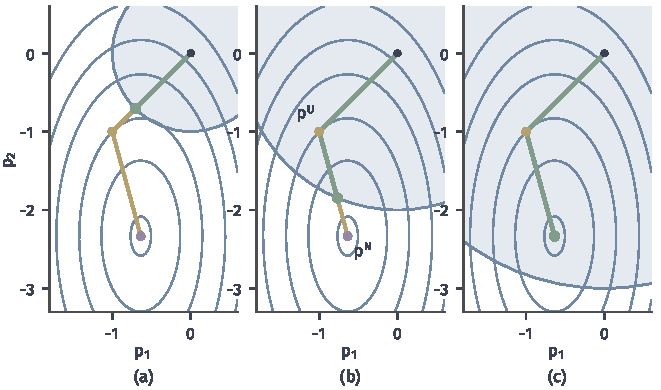
\includegraphics[width=112mm]{figures/05-optimization/02-smooth-optimization/matplotlib/tr-dogleg-path/figure.pdf}
 \caption{点$\bm{a}$的数据上半径分别为$1$、$2$、$3$的狗腿步。黄线是完整路径，绿线是实际走过的部分，绿点是得到的步。黄点是$\bm{p}^{\mathrm{U}}$，紫点是$\bm{p}^{\mathrm{N}}$，蓝线是模型等高线，浅蓝圆盘是信赖域。}
 \label{fig:tr-dogleg-path}
\end{BookInlineFigure}

狗腿步的预测下降不低于Cauchy步：若$\lVert\bm{p}^{\mathrm{U}}\rVert_2\geq\Delta$，两者相同；否则$\bm{p}^{\mathrm{U}}$本身就是Cauchy步，而由引理~\ref{lem:tr-dogleg-monotone}，狗腿步在路径上更靠后，模型值更低。所以它满足式~\eqref{eq:tr-sufficient-decrease}，$c_1=1/2$。

\paragraph{不正定时不能照搬}
上面的构造用到$\bm{B}\succ\bm{0}$：$\bm{p}^{\mathrm{N}}$要是模型的最小点，第二段上的模型才会下降。把原点的数据~\eqref{eq:tr-data-o}照搬进去，$\bm{g}^\top\bm{B}\bm{g}=2>0$，第一段还能算出$\bm{p}^{\mathrm{U}}=(-1,-1)^\top$，第二段却指向鞍点$(1,-1/3)^\top$。沿第二段模型上升，从$-1$一直升到$1/3$，图~\ref{fig:tr-dogleg-indefinite}画出了这一段。

\begin{BookInlineFigure}
 \centering
 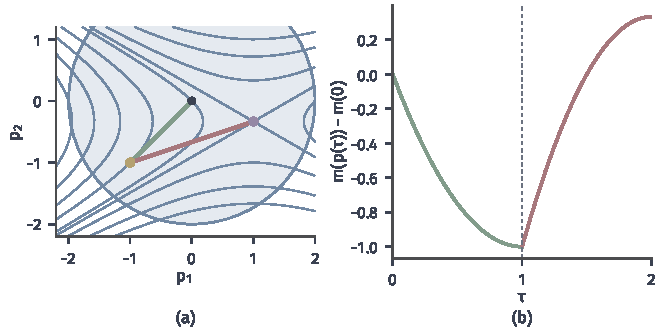
\includegraphics[width=112mm]{figures/05-optimization/02-smooth-optimization/matplotlib/tr-dogleg-indefinite/figure.pdf}
 \caption{把狗腿路径照搬到原点的不定模型上。(a)~模型等高线（蓝）与路径：绿色第一段走向黄点$\bm{p}^{\mathrm{U}}$，红色第二段走向模型的鞍点（紫）。(b)~沿路径的模型值，第二段（红）上升，路径上模型值的单调性失效。}
 \label{fig:tr-dogleg-indefinite}
\end{BookInlineFigure}

$\bm{B}$半正定且奇异时，$\bm{B}^{-1}$不存在，构造同样失效。这时要么先把$\bm{B}$修正成正定，要么换用下一小节的方法，后者不需要$\bm{B}$的任何分解。

\subsection{截断共轭梯度}
\label{sec:tr-truncated-cg}

\paragraph{主要思想}
Newton步是方程$\bm{B}\bm{p}=-\bm{g}$的解，也就是模型的驻点。第~\ref{chap:second-order-methods}章的Newton-CG用共轭梯度迭代近似解这个方程，只需要矩阵向量乘积。共轭梯度的推导和收敛性质可参考\BookChapterRef{chap:krylov-methods}{卷二第15章“Krylov子空间法”}，这里复述要用到的部分。

从$\bm{p}^{(0)}=\bm{0}$出发，记残差$\bm{r}^{(j)}=\bm{B}\bm{p}^{(j)}+\bm{g}$，它恰好是模型在$\bm{p}^{(j)}$处的梯度。内层迭代的上标用$j$，与外层的$t$区分。共轭梯度的递推是
\begin{equation}
 \begin{gathered}
  \alpha^{(j)}=\frac{\lVert\bm{r}^{(j)}\rVert_2^2}{\bm{d}^{(j)\top}\bm{B}\bm{d}^{(j)}},\qquad
  \bm{p}^{(j+1)}=\bm{p}^{(j)}+\alpha^{(j)}\bm{d}^{(j)},\\
  \bm{r}^{(j+1)}=\bm{r}^{(j)}+\alpha^{(j)}\bm{B}\bm{d}^{(j)},\\
  \beta^{(j)}=\frac{\lVert\bm{r}^{(j+1)}\rVert_2^2}{\lVert\bm{r}^{(j)}\rVert_2^2},\qquad
  \bm{d}^{(j+1)}=-\bm{r}^{(j+1)}+\beta^{(j)}\bm{d}^{(j)},
 \end{gathered}
 \label{eq:tr-cg}
\end{equation}
初始方向$\bm{d}^{(0)}=-\bm{g}$。$\alpha^{(j)}$是模型沿$\bm{d}^{(j)}$的精确一维最小点，所以每步模型值都下降。第一步恰好是$\bm{p}^{\mathrm{U}}$。

放进信赖域，只需要回答两个新问题：迭代走出半径了怎么办，遇到$\bm{B}$的非正曲率怎么办。\term{截断共轭梯度法}（truncated conjugate gradient method）的回答是：两种情况都沿当前方向走到边界，然后停止。

先看走出半径的情形。下面的引理说明，共轭梯度的迭代点离原点越来越远。一旦越出球，以后就不会回来，所以在第一次越界处截断不会错过后面的点。

\begin{lemma}[迭代点的长度递增]
 \label{lem:tr-cg-norm}
 设$\bm{g}\neq\bm{0}$，递推~\eqref{eq:tr-cg}进行到第$j$步，且此前各步曲率$\bm{d}^{(i)\top}\bm{B}\bm{d}^{(i)}>0$，残差非零。则
 \begin{equation}
  \lVert\bm{p}^{(j+1)}\rVert_2>\lVert\bm{p}^{(j)}\rVert_2.
  \label{eq:tr-cg-norm}
 \end{equation}
\end{lemma}

\begin{proof}
 残差相互正交，并且方向与残差张成同一子空间：
 \[
  \operatorname{span}\{\bm{d}^{(0)},\ldots,\bm{d}^{(j-1)}\}=\operatorname{span}\{\bm{r}^{(0)},\ldots,\bm{r}^{(j-1)}\}.
 \]
 这两条性质的归纳证明只用到递推~\eqref{eq:tr-cg}中的分母非零，不要求$\bm{B}$在全空间正定。由于$\bm{p}^{(j)}$是$\bm{d}^{(0)},\ldots,\bm{d}^{(j-1)}$的线性组合，所以$\langle\bm{p}^{(j)},\bm{r}^{(j)}\rangle=0$。

 用归纳法证明$\langle\bm{p}^{(j)},\bm{d}^{(j)}\rangle\geq0$。$j=0$时等于$0$。代入$\bm{d}^{(j+1)}$的定义，并用正交性，得到
 \[
  \langle\bm{p}^{(j+1)},\bm{d}^{(j+1)}\rangle=\beta^{(j)}\langle\bm{p}^{(j+1)},\bm{d}^{(j)}\rangle
  =\beta^{(j)}\bigl(\langle\bm{p}^{(j)},\bm{d}^{(j)}\rangle+\alpha^{(j)}\lVert\bm{d}^{(j)}\rVert_2^2\bigr),
 \]
 其中$\alpha^{(j)},\beta^{(j)}>0$，因此它非负。

 最后展开长度：
 \[
  \lVert\bm{p}^{(j+1)}\rVert_2^2=\lVert\bm{p}^{(j)}\rVert_2^2+2\alpha^{(j)}\langle\bm{p}^{(j)},\bm{d}^{(j)}\rangle+(\alpha^{(j)})^2\lVert\bm{d}^{(j)}\rVert_2^2>\lVert\bm{p}^{(j)}\rVert_2^2.
 \]
\end{proof}

再看非正曲率的情形。若$\bm{d}^{(j)\top}\bm{B}\bm{d}^{(j)}\leq0$，模型沿$\bm{d}^{(j)}$是凹的。由$\bm{r}^{(j)}$与$\bm{d}^{(j-1)}$正交可知模型沿$\bm{d}^{(j)}$的斜率为$-\lVert\bm{r}^{(j)}\rVert_2^2<0$，所以越往前走模型越低，应当一直走到边界。这正是第~\ref{sec:tr-model}节所说的利用负曲率。

三种停止各有含义，图~\ref{fig:tr-tcg-flow}是一步迭代的判断顺序。残差停止表示模型的驻点已经解得够准，判据沿用第~\ref{chap:second-order-methods}章非精确Newton法的形式：
\begin{equation}
 \lVert\bm{r}^{(j)}\rVert_2\leq\eta\lVert\bm{g}\rVert_2,\qquad\eta=\min\{0.1,\ \sqrt{\lVert\bm{g}\rVert_2}\}.
 \label{eq:tr-residual-stop}
\end{equation}

边界停止表示模型的最小点在球外。曲率停止表示模型沿这个方向没有最小点。后两条是信赖域给内层迭代新加的规则，Newton-CG遇到非正曲率时只能退回一个下降方向，交给线搜索。

\begin{BookInlineFigure}
 \centering
 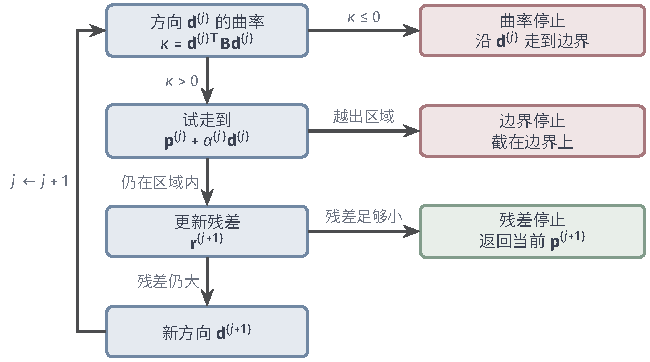
\includegraphics[width=110mm]{figures/05-optimization/02-smooth-optimization/tikz/tr-tcg-flow/figure.pdf}
 \caption{截断共轭梯度一次内层迭代的判断顺序。蓝框是普通的共轭梯度步骤，红框是信赖域带来的两种截断，绿框是沿用Newton-CG的残差停止。}
 \label{fig:tr-tcg-flow}
\end{BookInlineFigure}

\needspace{6\baselineskip}
\paragraph{变量}
下面的过程结合点$\bm{a}$的数据走一遍，要维护的量是：
\begin{itemize}
 \item $\bm{p}^{(j)}\in\mathbb{R}^n$：当前位移；
 \item $\bm{r}^{(j)}\in\mathbb{R}^n$：模型在$\bm{p}^{(j)}$处的梯度；
 \item $\bm{d}^{(j)}\in\mathbb{R}^n$：搜索方向；
 \item $\bm{B}\bm{d}^{(j)}\in\mathbb{R}^n$：一次矩阵向量乘积，是全部需要的曲率信息。
\end{itemize}

\paragraph{初始化}
取$\bm{p}^{(0)}=\bm{0}$，$\bm{r}^{(0)}=\bm{g}$，$\bm{d}^{(0)}=-\bm{g}$，容差$\eta$。例中半径$\Delta=2$，容差取$\eta=0.1$：
\[
 \bm{r}^{(0)}=\begin{bmatrix}7\\7\end{bmatrix},\qquad
 \bm{d}^{(0)}=\begin{bmatrix}-7\\-7\end{bmatrix},\qquad
 \eta\lVert\bm{g}\rVert_2\approx0.990.
\]

\paragraph{每轮更新}
第$j$轮依次执行以下步骤。

\begin{enumerate}
 \item 计算$\bm{B}\bm{d}^{(j)}$和曲率$\bm{d}^{(j)\top}\bm{B}\bm{d}^{(j)}$。若曲率不大于零，按式~\eqref{eq:tr-boundary-root}（其中$\bm{p}^{\mathrm{U}}$换成$\bm{p}^{(j)}$，$\bm{w}$换成$\bm{d}^{(j)}$）求出边界上的$\sigma$，返回$\bm{p}^{(j)}+\sigma\bm{d}^{(j)}$。例中第一轮
 \[
  \bm{B}\bm{d}^{(0)}=\begin{bmatrix}-77\\-21\end{bmatrix},\qquad
  \bm{d}^{(0)\top}\bm{B}\bm{d}^{(0)}=686>0.
 \]
 \item 由式~\eqref{eq:tr-cg}计算$\alpha^{(j)}$和试探点$\bm{p}^{(j)}+\alpha^{(j)}\bm{d}^{(j)}$。若试探点的长度不小于$\Delta$，同样求边界上的$\sigma$并返回。例中第一轮
 \[
  \alpha^{(0)}=\frac{98}{686}=\frac17,\qquad
  \bm{p}^{(1)}=\begin{bmatrix}-1\\-1\end{bmatrix},\qquad\lVert\bm{p}^{(1)}\rVert_2=\sqrt2<2.
 \]
 \item 由式~\eqref{eq:tr-cg}更新残差，若$\bm{r}^{(j+1)}$满足式~\eqref{eq:tr-residual-stop}，返回$\bm{p}^{(j+1)}$。例中第一轮
 \[
  \bm{r}^{(1)}=\begin{bmatrix}7\\7\end{bmatrix}+\frac17\begin{bmatrix}-77\\-21\end{bmatrix}=\begin{bmatrix}-4\\4\end{bmatrix},\qquad
  \lVert\bm{r}^{(1)}\rVert_2\approx5.66>0.990.
 \]
 \item 由式~\eqref{eq:tr-cg}计算$\beta^{(j)}$和新方向。例中第一轮
 \[
  \beta^{(0)}=\frac{32}{98}=\frac{16}{49},\qquad
  \bm{d}^{(1)}=\begin{bmatrix}4\\-4\end{bmatrix}+\frac{16}{49}\begin{bmatrix}-7\\-7\end{bmatrix}=\begin{bmatrix}12/7\\-44/7\end{bmatrix}.
 \]
\end{enumerate}

例中第二轮的曲率是
\[
 \bm{B}\bm{d}^{(1)}=\begin{bmatrix}132/7\\-132/7\end{bmatrix},\qquad
 \bm{d}^{(1)\top}\bm{B}\bm{d}^{(1)}=\frac{7392}{49}>0.
\]

于是$\alpha^{(1)}=32\cdot49/7392=7/33$。试探点正是Newton点，而它的长度约为$2.419$，超过了半径：
\[
 \bm{p}^{(1)}+\alpha^{(1)}\bm{d}^{(1)}=\begin{bmatrix}-7/11\\-7/3\end{bmatrix}.
\]

所以按边界停止。由式~\eqref{eq:tr-boundary-root}，边界上的$\sigma=7/52$，最终得到
\[
 \bm{p}=\begin{bmatrix}-1\\-1\end{bmatrix}+\frac{7}{52}\begin{bmatrix}12/7\\-44/7\end{bmatrix}=\begin{bmatrix}-10/13\\-24/13\end{bmatrix}.
\]

这和狗腿步完全相同，并不是巧合。二维时共轭梯度第一步到$\bm{p}^{\mathrm{U}}$，第二步到$\bm{p}^{\mathrm{N}}$，两段路径就是狗腿路径。维数大于$2$时两者不同：狗腿法从$\bm{p}^{\mathrm{U}}$直奔Newton点，截断共轭梯度沿途经过一串中间点，也不需要预先分解$\bm{B}$。半径若取$\Delta=3$，第二轮的试探点在球内，残差恰好为零，按残差停止，返回Newton步。

再用原点的数据~\eqref{eq:tr-data-o}、$\Delta=2$看曲率停止。第一轮的曲率$\bm{d}^{(0)\top}\bm{B}\bm{d}^{(0)}=2>0$，$\alpha^{(0)}=1$，试探点在球内，并有
\[
 \bm{p}^{(1)}=\begin{bmatrix}-1\\-1\end{bmatrix},\qquad
 \bm{r}^{(1)}=\begin{bmatrix}2\\-2\end{bmatrix},\qquad
 \bm{d}^{(1)}=\begin{bmatrix}-6\\-2\end{bmatrix}.
\]

第二轮的曲率是$-36+12=-24\leq0$，沿$\bm{d}^{(1)}$走到边界。由$\lVert\bm{p}^{(1)}+\sigma\bm{d}^{(1)}\rVert_2=2$得$20\sigma^2+8\sigma-1=0$，取正根$\sigma=1/10$，最终得到
\[
 \bm{p}=\begin{bmatrix}-8/5\\-6/5\end{bmatrix},\qquad\operatorname{pred}(\bm{p})=\frac{48}{25}=1.92.
\]
图~\ref{fig:tr-tcg-path}是这两次运行的轨迹。

\begin{BookInlineFigure}
 \centering
 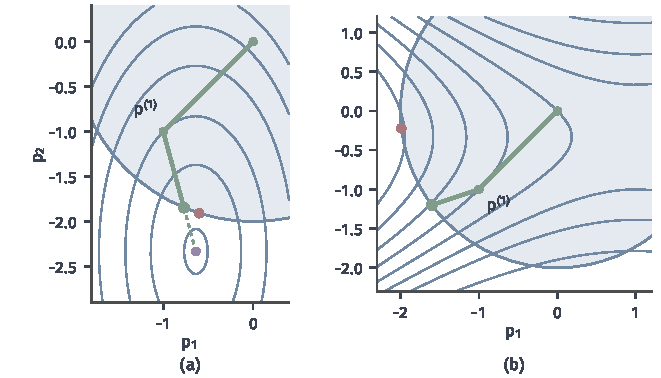
\includegraphics[width=112mm]{figures/05-optimization/02-smooth-optimization/matplotlib/tr-tcg-path/figure.pdf}
 \caption{截断共轭梯度的两次运行，绿线是迭代轨迹，绿色大点是返回的步，红点是子问题的全局解。(a)~点$\bm{a}$，第二轮越过边界而截断，虚线通向球外的Newton点（紫）。(b)~原点，第二轮遇到负曲率，沿方向走到边界。}
 \label{fig:tr-tcg-path}
\end{BookInlineFigure}

\paragraph{算法分析}
截断共轭梯度的第一轮要么到达$\bm{p}^{\mathrm{U}}$，要么在边界上截断，得到的都是Cauchy步，此后每一步模型值都不升高：普通步是精确一维最小化，边界截断发生在模型仍然下降的路段上。所以它的预测下降不低于Cauchy步，满足式~\eqref{eq:tr-sufficient-decrease}，$c_1=1/2$。

当$\bm{B}\succ\bm{0}$时还可以证明，截断共轭梯度的预测下降至少是全局解的一半，证明需要细致比较Krylov子空间上的子问题，篇幅较长，读者可查阅专门的信赖域文献。$\bm{B}$不定时没有这个保证：原点上它的预测下降只有$1.92$，全局解是$4.111$。它在图~\ref{fig:tr-tcg-path}(b)中沿方向$(-3,-1)^\top$走到边界，错过了曲率最负的方向$\bm{e}_1$。

表~\ref{tab:tr-subproblem-compare}汇总同一个模型上三种步和全局解的结果。

\begin{BookInlineTable}
 \centering
 \begin{tabular}{llrrrr}
  \toprule
  模型 & 量 & Cauchy步 & 狗腿步 & 截断共轭梯度 & 全局解\\
  \midrule
  点$\bm{a}$ & $\operatorname{pred}$ & $7.000$ & $9.941$ & $9.941$ & $10.115$\\
  & $\operatorname{ared}$ & $8.750$ & $10.764$ & $10.764$ & $10.515$\\
  原点 & $\operatorname{pred}$ & $1.000$ & 不适用 & $1.920$ & $4.111$\\
  & $\operatorname{ared}$ & $0.750$ & 不适用 & $0.282$ & $0.209$\\
  \bottomrule
 \end{tabular}
 \caption{半径$\Delta=2$时几种步的预测下降与实际下降。}
 \label{tab:tr-subproblem-compare}
\end{BookInlineTable}

二维例子看不出截断共轭梯度的省力之处。图~\ref{fig:tr-tcg-compare}取一个$n=200$的正定模型：Hessian向量乘积只用$9$次，预测下降就达到全局解的$98\%$，长度随次数严格增加，与引理~\ref{lem:tr-cg-norm}一致。这时狗腿法和精确求解都要作$200$阶矩阵的分解。

\begin{BookInlineFigure}
 \centering
 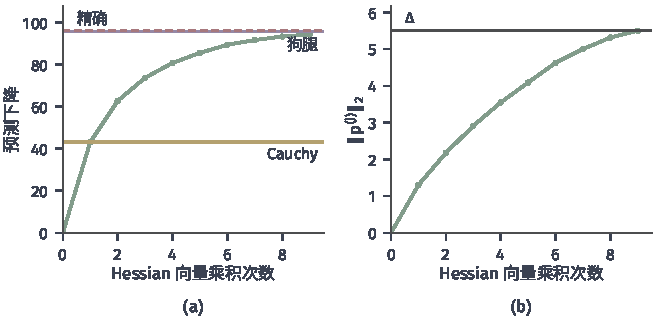
\includegraphics[width=112mm]{figures/05-optimization/02-smooth-optimization/matplotlib/tr-tcg-compare/figure.pdf}
 \caption{一个$n=200$的随机正定模型，特征值在$1$到$100$之间对数等距，$\Delta=5.5$，随机种子固定。(a)~截断共轭梯度（绿）的预测下降随矩阵向量乘积次数的变化，水平线依次为Cauchy步（黄）、狗腿步（紫）和全局解（红虚线）。(b)~迭代点长度（绿）递增，触及半径（深灰线）时停止。}
 \label{fig:tr-tcg-compare}
\end{BookInlineFigure}
